%%%%%%%%%%%%%%%%%%%%%%%%%%%%%%%%%%%%%%
% A presentation by Gilles Bertrand  %
% gilles.bertrand at ieee dot org   %
% December 2006            %
%%%%%%%%%%%%%%%%%%%%%%%%%%%%%%%%%%%%%%

\documentclass[pdf]{beamer}
\usetheme{Antibes}
\usecolortheme{dolphin}
\usepackage{time}       % date and time
\usepackage{graphicx}
\usepackage[T1]{fontenc}    % european characters
%\usepackage{courier}
\usepackage{amssymb,amsmath}  % use mathematical symbols
\usepackage{palatino}                  % use palatino as the default font
\setbeamercovered{transparent}
\setbeamertemplate{navigation symbols}{}
\begin{document}

% here you define the information that will be displayed in the title/cover page
\title[Lego Racing Team]{Lego Racing Team\\\small{Final presentation}}
%\subtitle {subtitle}
\author[...]{Christian Dietz, Jan Seeger, Julian Tatsch \\ Rainer Sch\"{o}nberger, Wenwen Chen\\}
\date{15. Juli 2013}

% this is used in the pdf information
\subject{Final presentation}

% here you build the title page
\frame{
 \titlepage
}

% outline
%\AtBeginSection[]
%{
% \begin{frame}
%  \frametitle{Kapitel\"{u}bersicht}
%  \small
%  \tableofcontents[currentsection,hideothersubsections]
%  \normalsize
% \end{frame}
%}


\section{Recap}
\subsection{Motivation}
\begin{frame}
\frametitle{Motivation}
\begin{exampleblock}{Build a high speed capable car}
\begin{itemize}
  \item with flexible heterogenous user interfaces (Android, Wiimote, Laptop)
  \item assist the user (traction control, obstacle avoidance, emergency brake)
  \item leverage the power of the FPGA where suitable
\end{itemize}
\end{exampleblock}
\end{frame}

\section{Recap}
\subsection{Architecture}
\begin{frame}
\frametitle{Architecture}
  \begin{center}
  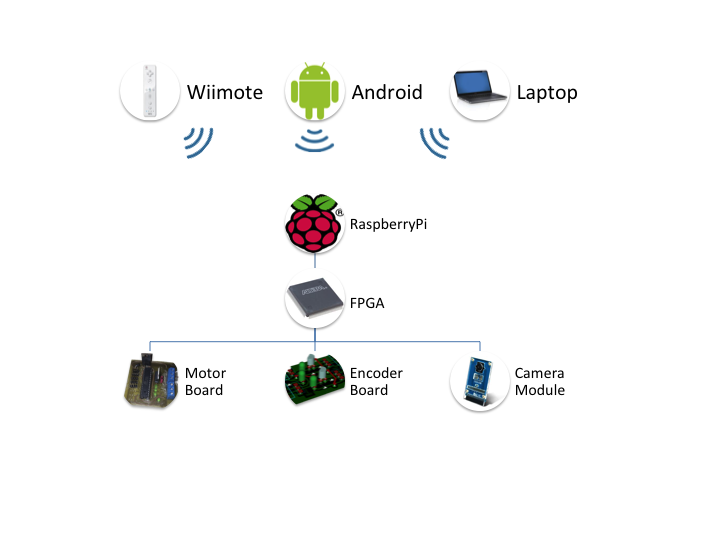
\includegraphics[width = \textwidth]{pics/architecture.png}
  \end{center}
\end{frame}

\section{Status Update}
\subsection{Hardware}
\begin{frame}
\frametitle{Hardware}
\begin{exampleblock}{Update}
\begin{itemize}
  \item Integrated new high power wireless access point
  \item Built second servo board to parallelize development on RASPI and FPGA
  \item Connect all components with pin-socket connectors for faster reconnection
\end{itemize}
\end{exampleblock}
\end{frame}

\section{Status Update}
\subsection{FPGA}
\begin{frame}
\frametitle{FPGA}
\begin{exampleblock}{Update}
\begin{itemize}
  \item Implemented reading out the encoders
  \item Implemented I2C protocol for motor control
  \item Implemented SPI protocol to communicate with top-level (RASPI)
  \item Implemented motor speed control
\end{itemize}
\end{exampleblock}
\end{frame}

\section{Status Update}
\subsection{FPGA}
\begin{frame}
\frametitle{FPGA}
  \begin{center}
  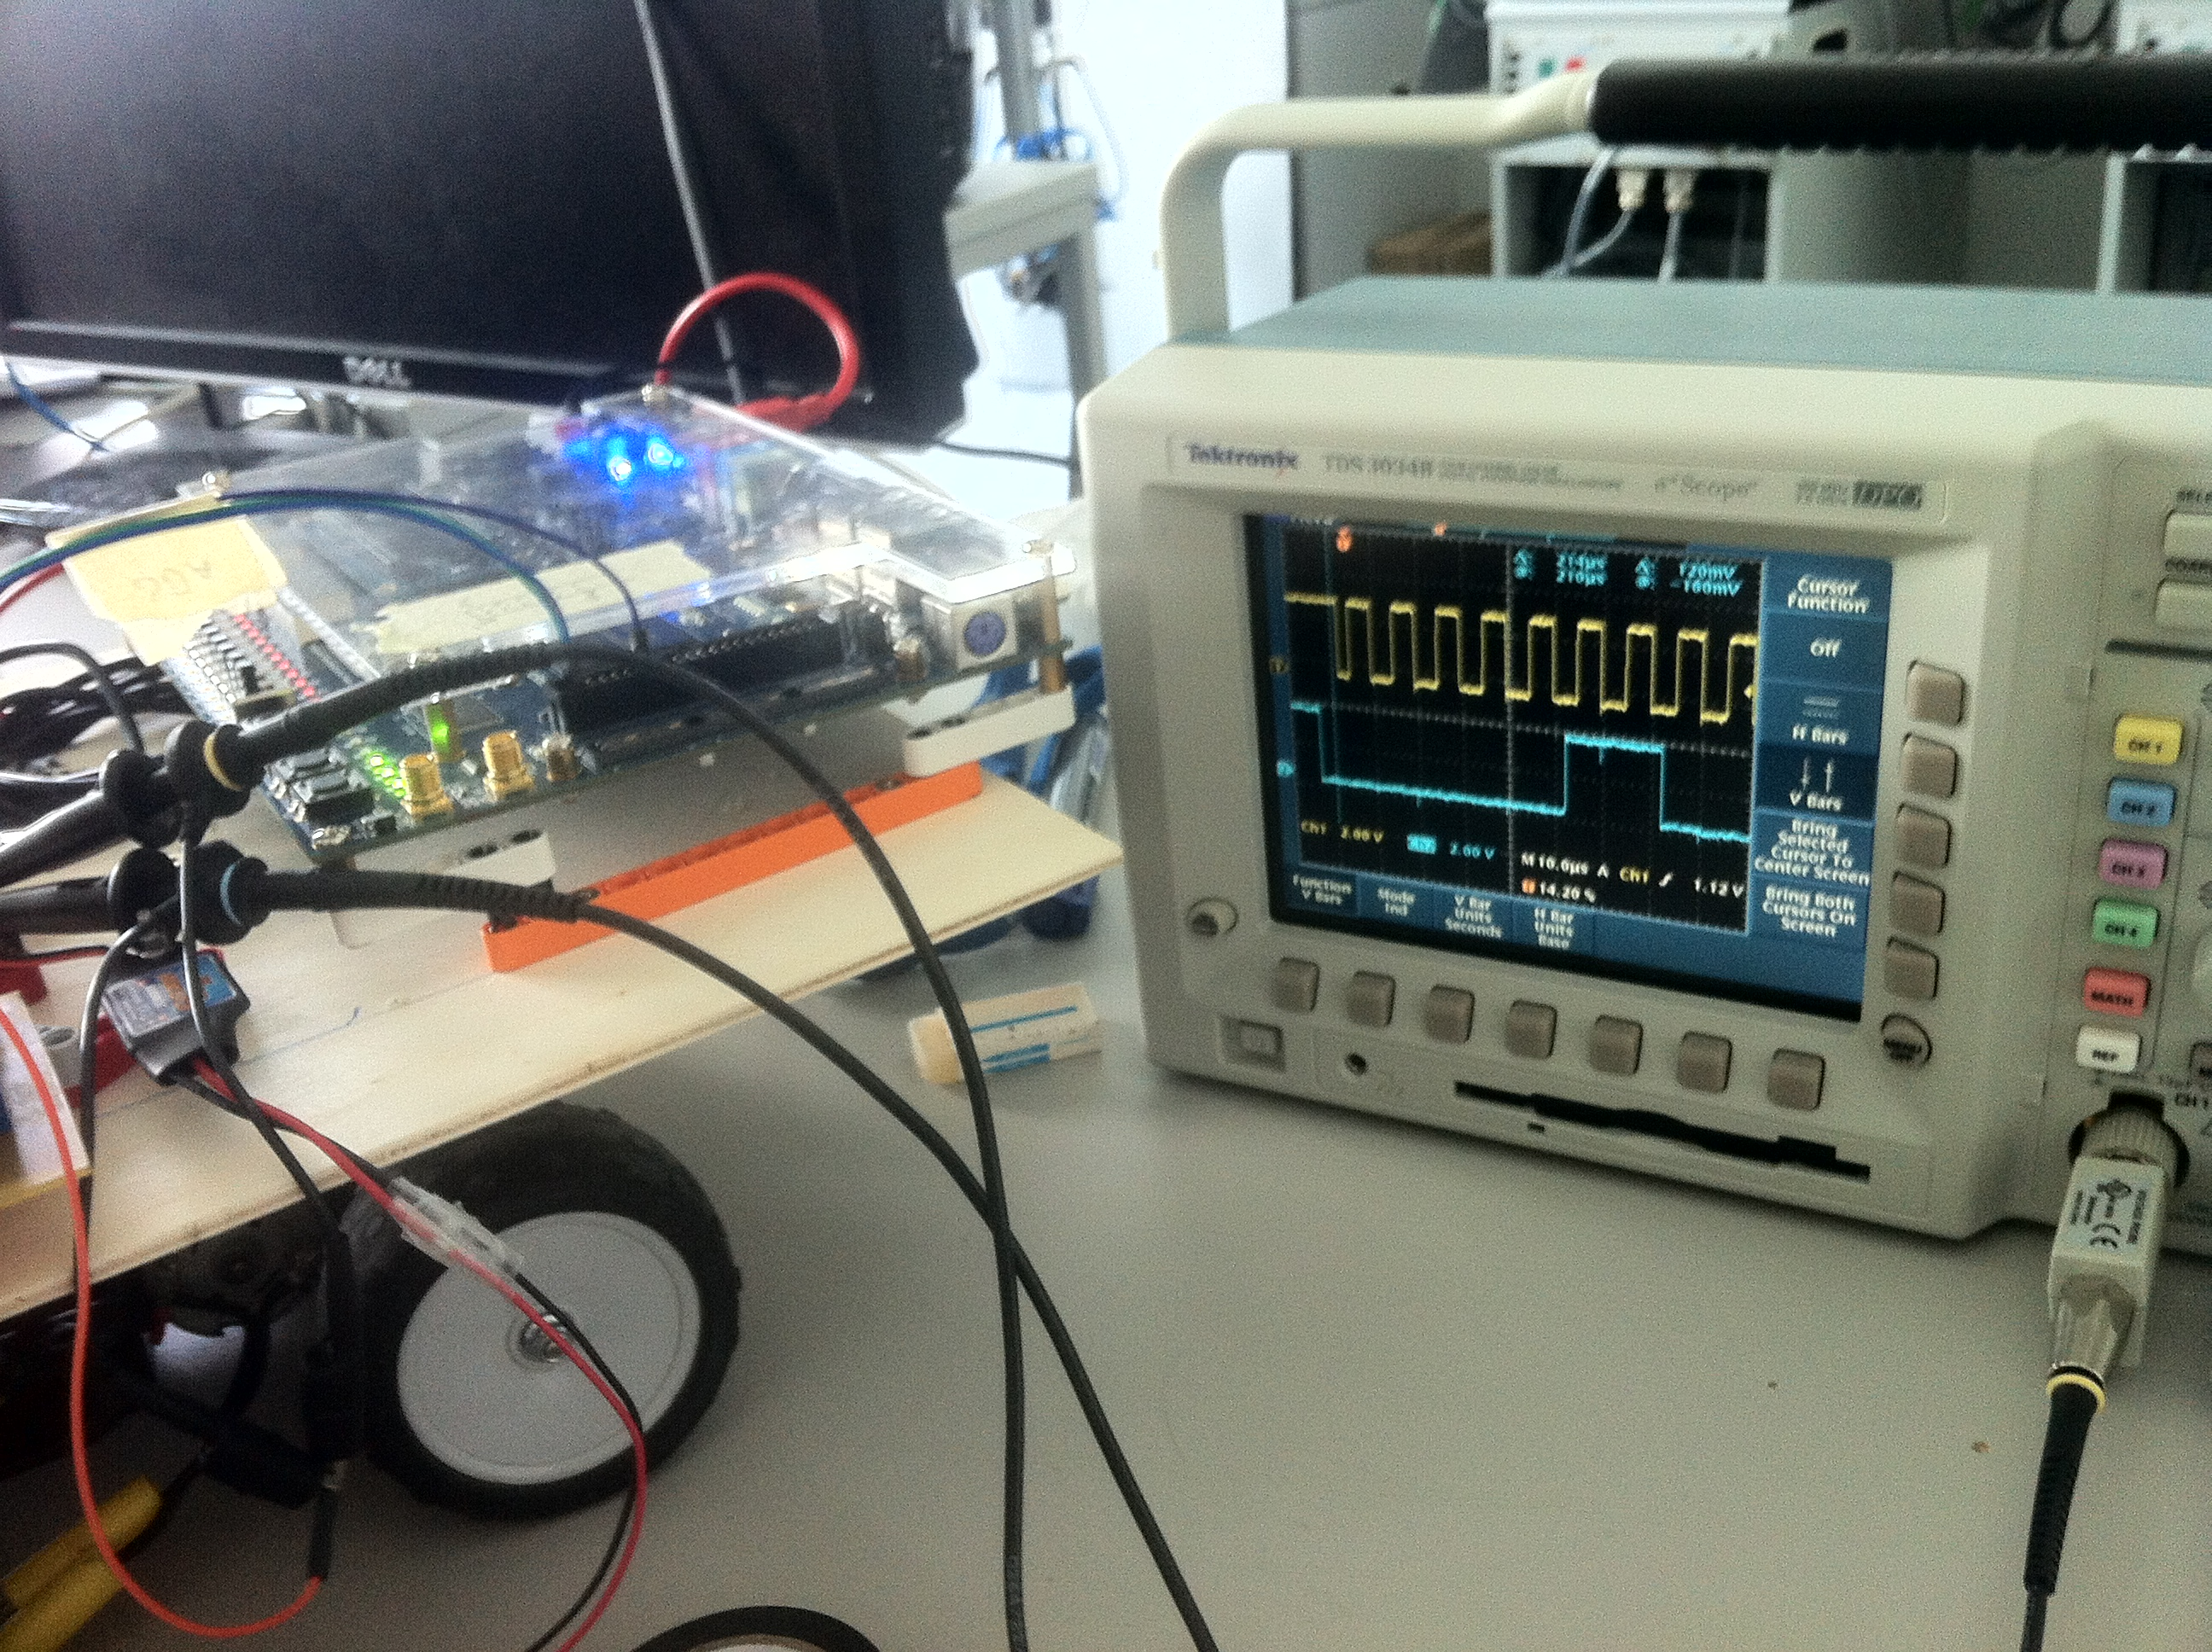
\includegraphics[width = \textwidth]{pics/i2c_am_oszi.JPG}
  \end{center}
\end{frame}

\section{Status Update}
\subsection{RASPI}
\begin{frame}
\frametitle{Raspi}
\begin{exampleblock}{Update}
\begin{itemize}
  \item Implemented SPI interface to FPGA
  \item Moved some general input processing to the RASPI
\end{itemize}
\end{exampleblock}
\end{frame}

\section{Next steps}
\begin{frame}
\frametitle{Next steps}
\begin{exampleblock}{Plan}
\begin{itemize}
\item Get the camera to work on FPGA 
\item Implement laser scanning algorithm on FPGA
\item Implement obstacle avoidance on RASPI
\item Implement communication between FPGA and RASPI
\end{itemize}
\end{exampleblock}
\end{frame}

\section{Lessons learned}
\begin{frame}
\frametitle{Lessons learned}
\begin{exampleblock}{}
\begin{itemize}
\item Implementation on the FPGA extremely time-consuming
\item Simuluated FPGA != real FPGA
\item Debugging on the FPGA is tedious, memory oscilloscopes or logic analyzer are of great help  
\item Watch out for endianness when connecting different systems
\end{itemize}
\end{exampleblock}
\end{frame}

\end{document}

%%% Local Variables:
%%% mode: latex
%%% TeX-master: t
%%% End: